QUIC, tout comme TCP, est un protocole de communication pair à pair assurant l'intégrité des communications.
QUIC est conçu pour assurer que tous les paquets réseaux d'une communication arrivent dans l'ordre et inaltérés.
À l'instar de TCP, QUIC fournit un contrôle de congestion permettant d'obtenir des débits optimaux sans saturer le réseau.
Afin de s'intégrer aisément avec les systèmes d'exploitation actuels et les pare-feu, QUIC est construit au-dessus d'UDP, ainsi, bien que QUIC soit un remplacement de TCP, il se situe un niveau au-dessus dans le modèle en couche, au niveau de l'application.

\begin{figure}[H]
    \centering
    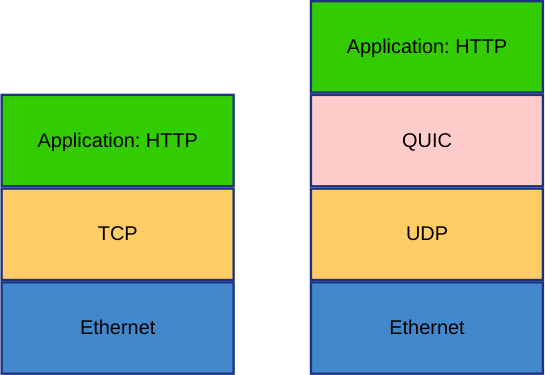
\includegraphics[height=0.20\textheight]{figures/network_layers.png}
    \caption{Modèle en couche - QUIC est construit sur UDP}
\end{figure}

Parmi les différences entre QUIC et TCP, on notera que QUIC chiffre toutes les communications, même les acquittements sont chiffrés de sorte que toute communication soit intégralement opaque pour un observateur extérieur. Un autre avantage majeur de QUIC est la possibilité de multiplexer différents flux sur une même connexion. En théorie cela permet de ne négocier la clef de chiffrement qu'une seule fois, réduisant ainsi la charge sur les serveurs HTTP/3. En effet, une simple recherche google génère aujourd'hui une cinquantaine de requêtes HTTP, chaque requête négociant une nouvelle clef de chiffrement. Intuitivement, pour des services comme YouTube, le nombre de requêtes est encore plus élevé, d'où l'intérêt de multiplexer les flux.
Pour finir sur les différences, QUIC apporte beaucoup plus de contrôle sur les paramètres de la connexion, permettant ainsi de le configurer pour des applications très différentes, du streaming haut débit sur YouTube à des connexions à très grande latence, comme une communication avec Mars.

Malgré tous ces avantages, QUIC a un défaut majeur, toutes les implémentations actuelles consomment énormément de puissance de calcul, bien plus que TCP.
Il y a plusieurs raisons à cela. D'une part, les implémentations de QUIC sont très jeunes et n'ont pas eu le temps d'être optimisées, contrairement aux implémentations de TCP qui ont reçu des décennies d'améliorations, l'implémentation de TCP dans Linux date de 1992\up{\cite{linux-first-tcp}}.
D'autre part, QUIC est fait pour être implémenté au-dessus d'UDP, du côté application, tandis que TCP est implémenté dans le kernel. Pour éviter que les trames IP soient fragmentées par les routeurs, les paquets que l'on génère ne doivent pas dépasser les 1400 octets. Travailler sur de si petits paquets rend la cryptographie plus intensive et nécessite de nombreux appels kernel, ce qui explique majoritairement les écarts de performances entre QUIC et TCP.

C'est pour contrebalancer ce défaut que beaucoup de recherches actuelles sur les implémentations de QUIC essayent de réduire l'utilisation du processeur par divers moyens, ce qui en pratique demande généralement d'ajouter des mécanismes dans le protocole QUIC pour traiter les données différemment.
QUIC VReverso et son implémentation frochet/quiceh est une de ces tentatives d'amélioration, l'idée étant ici de réduire le nombre de copies des données, ce qui consomme une part non négligeable du temps du processeur.

frochet/quiceh étant écrit en langage Rust, ne pouvait pas être intégré dans le client HTTP cURL qui est écrit en langage C. Il fallait donc écrire une FFI (Function to Function Interface), c'est à dire un morceau de code à l'interface entre les 2 langages qui convertit les données dans le format d'un langage vers le format de l'autre.
C'est le premier travail qui a été effectué.